\documentclass{article}
\usepackage[margin=1in]{geometry}
\usepackage{amsmath,amsthm,amssymb}
\usepackage{bbm,enumerate,mathtools}
\usepackage{tikz,pgfplots}
\usepackage{chessboard}
\usepackage[hidelinks]{hyperref}
\usepackage{multicol} % Problem 35

\newenvironment{question}{\begin{trivlist}\item[\textbf{Question.}]}{\end{trivlist}}
\newenvironment{note}{\begin{trivlist}\item[\textbf{Note.}]}{\end{trivlist}}
\newenvironment{references}{\begin{trivlist}\item[\textbf{References.}]}{\end{trivlist}}
\newenvironment{related}{\begin{trivlist}\item[\textbf{Related.}]\end{trivlist}\begin{enumerate}}{\end{enumerate}}


\begin{document}
\rating{4}{2}
Consider folding a strip of $n$ equilateral triangles down to 1 triangle in as
few moves as possible.
\begin{figure}[!h]
  \centering
  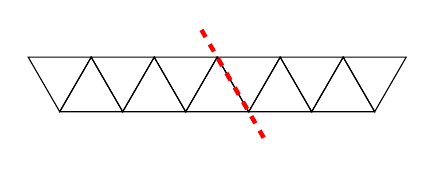
\begin{tikzpicture}[scale = 0.8]
    % right side up
    \foreach \x/\y in {0/0, 1/0, 2/0, 3/0, 4/0} {
      \draw ({\x + 0}, {sqrt(3)/2 * \y + 0})--({\x + 1/2}, {sqrt(3)/2 * \y + sqrt(3)/2})--({\x + 1},{sqrt(3)/2 * \y + 0})--cycle;
    }
    \foreach \x/\y in {-0.5/1, 0.5/1, 1.5/1, 2.5/1, 3.5/1, 4.5/1} {
      \draw (\x, {sqrt(3)/2 * \y + 0})--({\x + 0.5}, {sqrt(3)/2 * \y - sqrt(3)/2})--({\x + 1},{sqrt(3)/2 * \y + 0})--cycle;
    }
    \draw[ultra thick, red, dashed] (2.25, {sqrt(3)/2 * 1.5})--(3.25,{sqrt(3)/2 * -1/2});
  \end{tikzpicture}
  \hspace{1cm}
  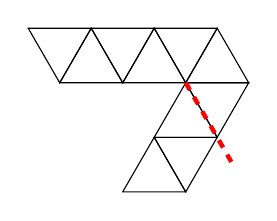
\begin{tikzpicture}[scale = 0.8]
    % right side up
    \foreach \x/\y in {0/0, 1/0, 2/0, 1.5/-1, 1/-2} {
      \draw ({\x + 0}, {sqrt(3)/2 * \y + 0})--({\x + 1/2}, {sqrt(3)/2 * \y + sqrt(3)/2})--({\x + 1},{sqrt(3)/2 * \y + 0})--cycle;
    }
    \foreach \x/\y in {-0.5/1, 0.5/1, 1.5/1, 2/0, 1.5/-1} {
      \draw (\x, {sqrt(3)/2 * \y + 0})--({\x + 0.5}, {sqrt(3)/2 * \y - sqrt(3)/2})--({\x + 1},{sqrt(3)/2 * \y + 0})--cycle;
    }
    \draw[ultra thick, red, dashed] (2, 0)--(2.75,{sqrt(3)/2 * -3/2});
  \end{tikzpicture}
  \hspace{1cm}
  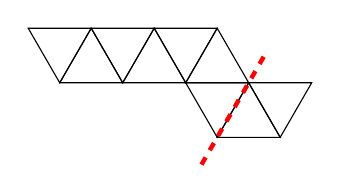
\begin{tikzpicture}[scale = 0.8]
    % right side up
    \foreach \x/\y in {0/0, 1/0, 2/0, 2.5/-1} {
      \draw ({\x + 0}, {sqrt(3)/2 * \y + 0})--({\x + 1/2}, {sqrt(3)/2 * \y + sqrt(3)/2})--({\x + 1},{sqrt(3)/2 * \y + 0})--cycle;
    }
    \foreach \x/\y in {-0.5/1, 0.5/1, 1.5/1, 2/0, 3/0} {
      \draw (\x, {sqrt(3)/2 * \y + 0})--({\x + 0.5}, {sqrt(3)/2 * \y - sqrt(3)/2})--({\x + 1},{sqrt(3)/2 * \y + 0})--cycle;
    }
    \draw[ultra thick, red, dashed] ({2.5 - 1/4}, {-sqrt(3)/2 - sqrt(3)/4})--({3 + 1/4}, {sqrt(3)/4});
  \end{tikzpicture}
  \vspace{0.5cm}

  \noindent
  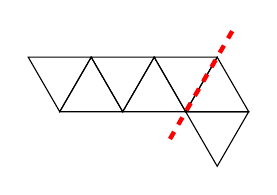
\begin{tikzpicture}[scale = 0.8]
    % right side up
    \foreach \x/\y in {0/0, 1/0, 2/0} {
      \draw ({\x + 0}, {sqrt(3)/2 * \y + 0})--({\x + 1/2}, {sqrt(3)/2 * \y + sqrt(3)/2})--({\x + 1},{sqrt(3)/2 * \y + 0})--cycle;
    }
    \foreach \x/\y in {-0.5/1, 0.5/1, 1.5/1, 2/0} {
      \draw (\x, {sqrt(3)/2 * \y + 0})--({\x + 0.5}, {sqrt(3)/2 * \y - sqrt(3)/2})--({\x + 1},{sqrt(3)/2 * \y + 0})--cycle;
    }
    \draw[ultra thick, red, dashed] ({2 - 1/4}, {-sqrt(3)/4})--(2.75,{sqrt(3)/2 + sqrt(3)/4});
  \end{tikzpicture}
  \hspace{1cm}
  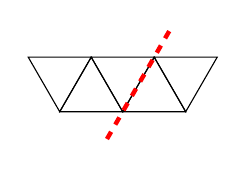
\begin{tikzpicture}[scale = 0.8]
    % right side up
    \foreach \x/\y in {0/0, 1/0} {
      \draw ({\x + 0}, {sqrt(3)/2 * \y + 0})--({\x + 1/2}, {sqrt(3)/2 * \y + sqrt(3)/2})--({\x + 1},{sqrt(3)/2 * \y + 0})--cycle;
    }
    \foreach \x/\y in {-0.5/1, 0.5/1, 1.5/1} {
      \draw (\x, {sqrt(3)/2 * \y + 0})--({\x + 0.5}, {sqrt(3)/2 * \y - sqrt(3)/2})--({\x + 1},{sqrt(3)/2 * \y + 0})--cycle;
    }
    \draw[ultra thick, red, dashed] ({1-1/4}, {-sqrt(3)/4})--(1.75,{sqrt(3)/2 + sqrt(3)/4});
  \end{tikzpicture}
  \hspace{1cm}
  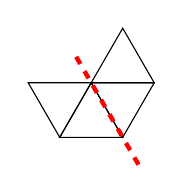
\begin{tikzpicture}[scale = 0.8]
    % right side up
    \foreach \x/\y in {0/0, 0.5/1} {
      \draw ({\x + 0}, {sqrt(3)/2 * \y + 0})--({\x + 1/2}, {sqrt(3)/2 * \y + sqrt(3)/2})--({\x + 1},{sqrt(3)/2 * \y + 0})--cycle;
    }
    \foreach \x/\y in {-0.5/1, 0.5/1} {
      \draw (\x, {sqrt(3)/2 * \y + 0})--({\x + 0.5}, {sqrt(3)/2 * \y - sqrt(3)/2})--({\x + 1},{sqrt(3)/2 * \y + 0})--cycle;
    }
    \draw[ultra thick, red, dashed] (1.25, {-sqrt(3)/4})--(0.25,{sqrt(3)/2 + sqrt(3)/4});
  \end{tikzpicture}
  \hspace{1cm}
  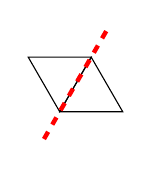
\begin{tikzpicture}[scale = 0.8]
    % right side up
    \foreach \x/\y in {0/0} {
      \draw ({\x + 0}, {sqrt(3)/2 * \y + 0})--({\x + 1/2}, {sqrt(3)/2 * \y + sqrt(3)/2})--({\x + 1},{sqrt(3)/2 * \y + 0})--cycle;
    }
    \foreach \x/\y in {-0.5/1} {
      \draw (\x, {sqrt(3)/2 * \y + 0})--({\x + 0.5}, {sqrt(3)/2 * \y - sqrt(3)/2})--({\x + 1},{sqrt(3)/2 * \y + 0})--cycle;
    }
    \draw[ultra thick, red, dashed] (-1/4, {-sqrt(3)/4})--(3/4,{3/4*sqrt(3)});
  \end{tikzpicture}
  \hspace{1cm}
  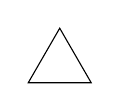
\begin{tikzpicture}[scale = 0.8]
    % right side up
    \foreach \x/\y in {0/0} {
      \draw ({\x + 0}, {sqrt(3)/2 * \y + 0})--({\x + 1/2}, {sqrt(3)/2 * \y + sqrt(3)/2})--({\x + 1},{sqrt(3)/2 * \y + 0})--cycle;
    }
  \end{tikzpicture}
  \caption{
    An example demonstrating that $a(11) \leq 7$.
  }
\end{figure}
\begin{question}
  How many folds are required to fold a strip of $n$ triangles down to one?
\end{question}
\begin{related}
  \item What if other $n$-iamonds are considered? Which $n$-iamond takes the
  greatest number of folds?
  \item Does there exist a family of $n$-iamonds that require more than
    $\mathcal O(\log_2(n))$ folds?
  \item Given an $n$-iamond uniformly at random, what's the expected value of
  the number of folds required?
  \item What if you must fold a single cell versus across a line?
  \item Consider the graded poset of polyiamonds given by the covering relation
  $x \lessdot y$ if $y$ is one fold away from $x$. How many polyiamonds have
  rank $n$?
  \begin{itemize}
    \item There is at least one $2^k$-iamond with rank $k$. How many
    $2^k$-iamonds are there with rank $k$?
    \item What's the second largest polyiamond of rank $k$?
    \item What's the smallest polyiamond of rank $k$?
    \item Is this poset Sperner?
  \end{itemize}
  \item Is there a sensible way to generalize this construction to other polyforms?
\end{related}

\end{document}
